\documentclass[aspectratio=169]{beamer}

\usetheme{metropolis}
\usepackage{booktabs}
\usepackage{graphicx}
\usepackage{amsmath}
\usepackage{xcolor}
\usepackage{colortbl}
\usepackage{array}
\usepackage{comment}

% Color palette matching the frontier plots
\definecolor{precovid}{RGB}{29,158,117}   % teal  #1D9E75
\definecolor{postcovid}{RGB}{83,74,183}   % purple #534AB7
\definecolor{darkgray}{RGB}{50,50,50}

\setbeamercolor{progress bar}{fg=postcovid}
\setbeamercolor{frametitle}{bg=darkgray}
\setbeamercolor{alerted text}{fg=postcovid}

\title{Efficient Frontier Shift:\\Pre- vs.\ Post-COVID Indian Equities}
\subtitle{IQF Midterm Project}
\author{Viraat Arora \and Yash Khaitan \and Dersh Savla}
\date{2026}

\begin{document}

% ─────────────────────────────────────────────
\maketitle

% ─────────────────────────────────────────────
\begin{frame}{Research Question}
  \begin{block}{}
    \centering\large
    Does the efficient frontier for Indian equities shift meaningfully\\
    between \textbf{pre-COVID (2015--2020)} and \textbf{post-COVID (2021--2024)},\\
    and what structural forces drive the shift?
  \end{block}

  \vspace{1em}
  \textbf{Why it matters}
  \begin{itemize}
    \item COVID was a sharp structural break in global markets
    \item India's equity market saw unprecedented post-pandemic stimulus and sectoral rotation
    \item A shift in the frontier implies a change in the \emph{fundamental} risk-return trade-off available to investors
  \end{itemize}
\end{frame}
% ─────────────────────────────────────────────
\begin{frame}{Motivation}
  
  \vspace{0.3em}
  \small
  \begin{columns}[T]
    \column{0.48\textwidth}
      \textbf{Policy \& Market Structure}
      \begin{itemize}
        \item \textbf{Unprecedented stimulus}: RBI cut repo rate from 5.15\% to 4.0\%; massive OMO and LTRO liquidity injections
        \item \textbf{Digital transformation}: COVID accelerated e-commerce, fintech, remote work --- reshaping sectoral weights
        \item \textbf{Retail investor boom}: Demat accounts grew from 4 crore (2019) to 14+ crore (2024); SIP flows surged
      \end{itemize}

    \column{0.48\textwidth}
      \textbf{India-Specific Factors}
      \begin{itemize}
        \item \textbf{China+1 strategy}: FII inflows as India became alternative manufacturing hub
        \item \textbf{PLI schemes}: Production-linked incentives reshaping industrial landscape
        \item \textbf{Fastest-growing major economy}: Post-COVID growth trajectory diverged from developed markets
      \end{itemize}
  \end{columns}
\end{frame}

% ─────────────────────────────────────────────
\begin{frame}{Dataset}

      \textbf{Universe}
      \begin{itemize}
        \item 45 stocks from NIFTY 50 (as of Jan 1, 2015)
        \item Source: Yahoo Finance 
      \end{itemize}
      \vspace{0.8em}
      \textbf{Periods}
      \begin{itemize}
        \item Pre-COVID: Jan 2015 -- Jan 2020
        \item Post-COVID: Jul 2021 -- Dec 2024
        \item Analyzed at daily \& weekly frequency
      \end{itemize}

      \textbf{Estimation}
      \begin{itemize}
        \item Annualized Returns ($\times 252$ daily, $\times 52$ weekly)
        \item Ledoit-Wolf shrinkage covariance
        \item Risk-free rate: RBI 91-day T-Bill yield (pre: 6.54\%, post: 5.78\%)
      \end{itemize}
      \vspace{0.4em}

\end{frame}

% ─────────────────────────────────────────────
\begin{frame}{NIFTY 50 Index: 2015--2024}
  \begin{center}
    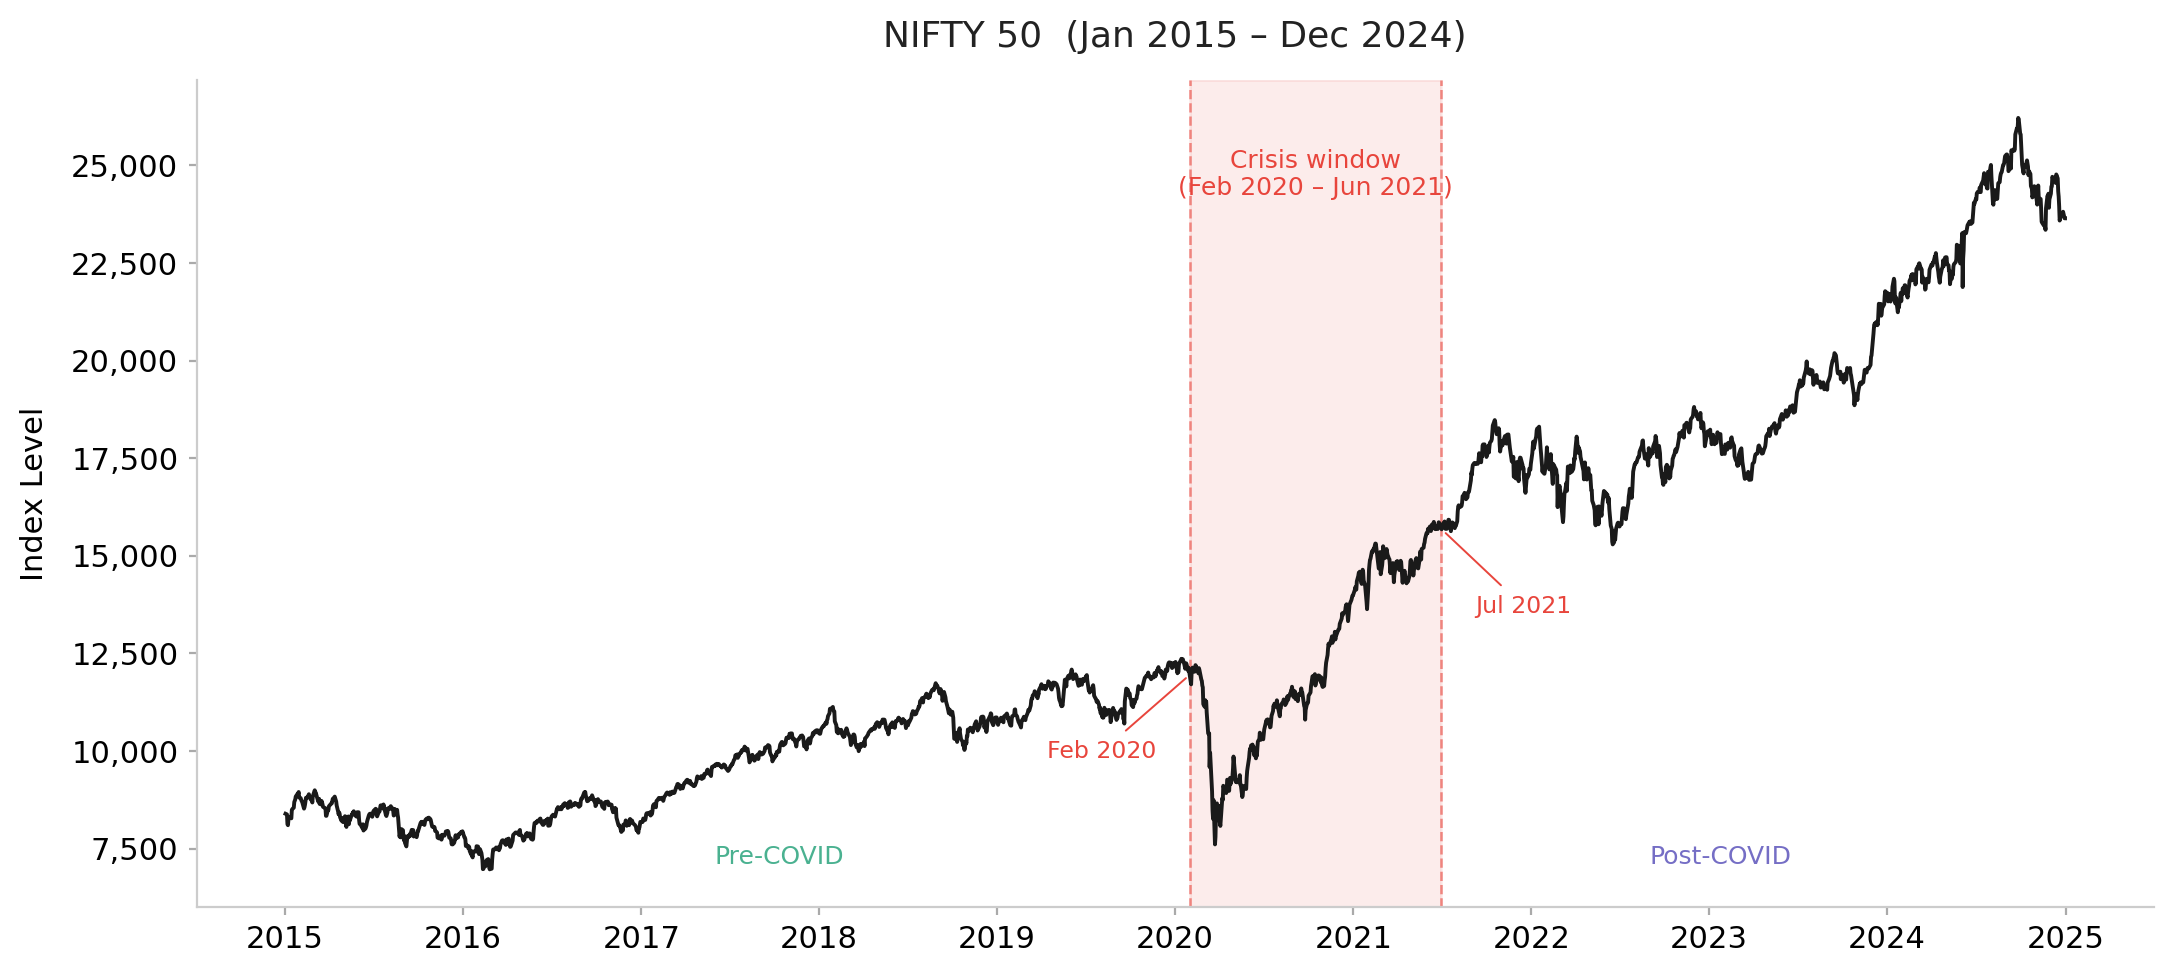
\includegraphics[width=0.90\textwidth]{Figures/nifty50_timeline.png}
  \end{center}
  \vspace{-0.6em}
  \small
  \begin{itemize}
    \item NIFTY fell $\approx$\,26\% peak-to-trough (Feb--Mar 2020); the crisis window (shaded) is \emph{excluded} from both estimation periods
    \item Post-COVID window captures a clean bull-market regime, free of crash-induced distortions
  \end{itemize}
\end{frame}

% ─────────────────────────────────────────────
\begin{frame}{Methodology}
  \begin{enumerate}
    \item \textbf{Compute statistics} --- annualized returns; Ledoit-Wolf shrinkage applied to $\boldsymbol{\Sigma}$ for each period
    \vspace{0.4em}
    \vspace{0.4em}
    \item \textbf{Trace the efficient frontier} --- Solve the minimization problem for multiple points to trace the efficient frontier
      \[
        \min_{\mathbf{w}}\; \mathbf{w}^\top \boldsymbol{\Sigma}\, \mathbf{w}
        \quad\text{s.t.}\quad \mathbf{w}^\top \boldsymbol{\mu} = \mu^*,\;
        \mathbf{w}^\top \mathbf{1} = 1,\; \mathbf{w} \ge 0
      \]
      sweeping $\mu^*$ from GMV to the highest-return asset
    \vspace{0.4em}
    \item \textbf{Tangency portfolio} --- maximize Sharpe ratio with RBI T-bill as $r_f$; compare pre vs.\ post weights
  \end{enumerate}
\end{frame}

% ─────────────────────────────────────────────
\begin{frame}{Efficient Frontier --- Daily \& Weekly}
  \begin{columns}[T]
    \column{0.5\textwidth}
      \centering
      \textbf{Daily}\\[0.4em]
      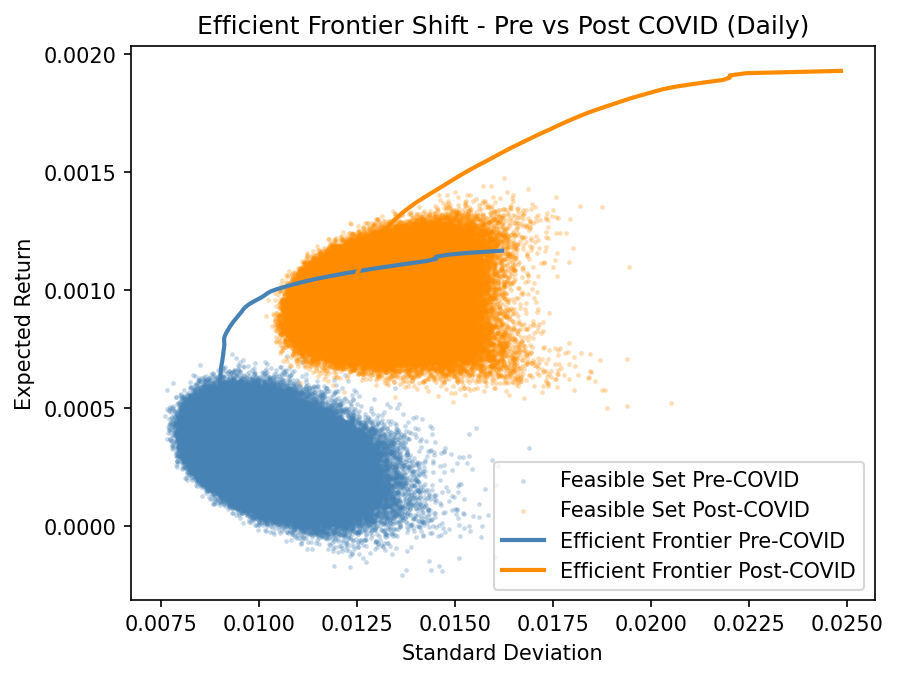
\includegraphics[width=\textwidth]{Figures/frontier_combined_daily.png}

    \column{0.5\textwidth}
      \centering
      \textbf{Weekly} \\[0.4em]
      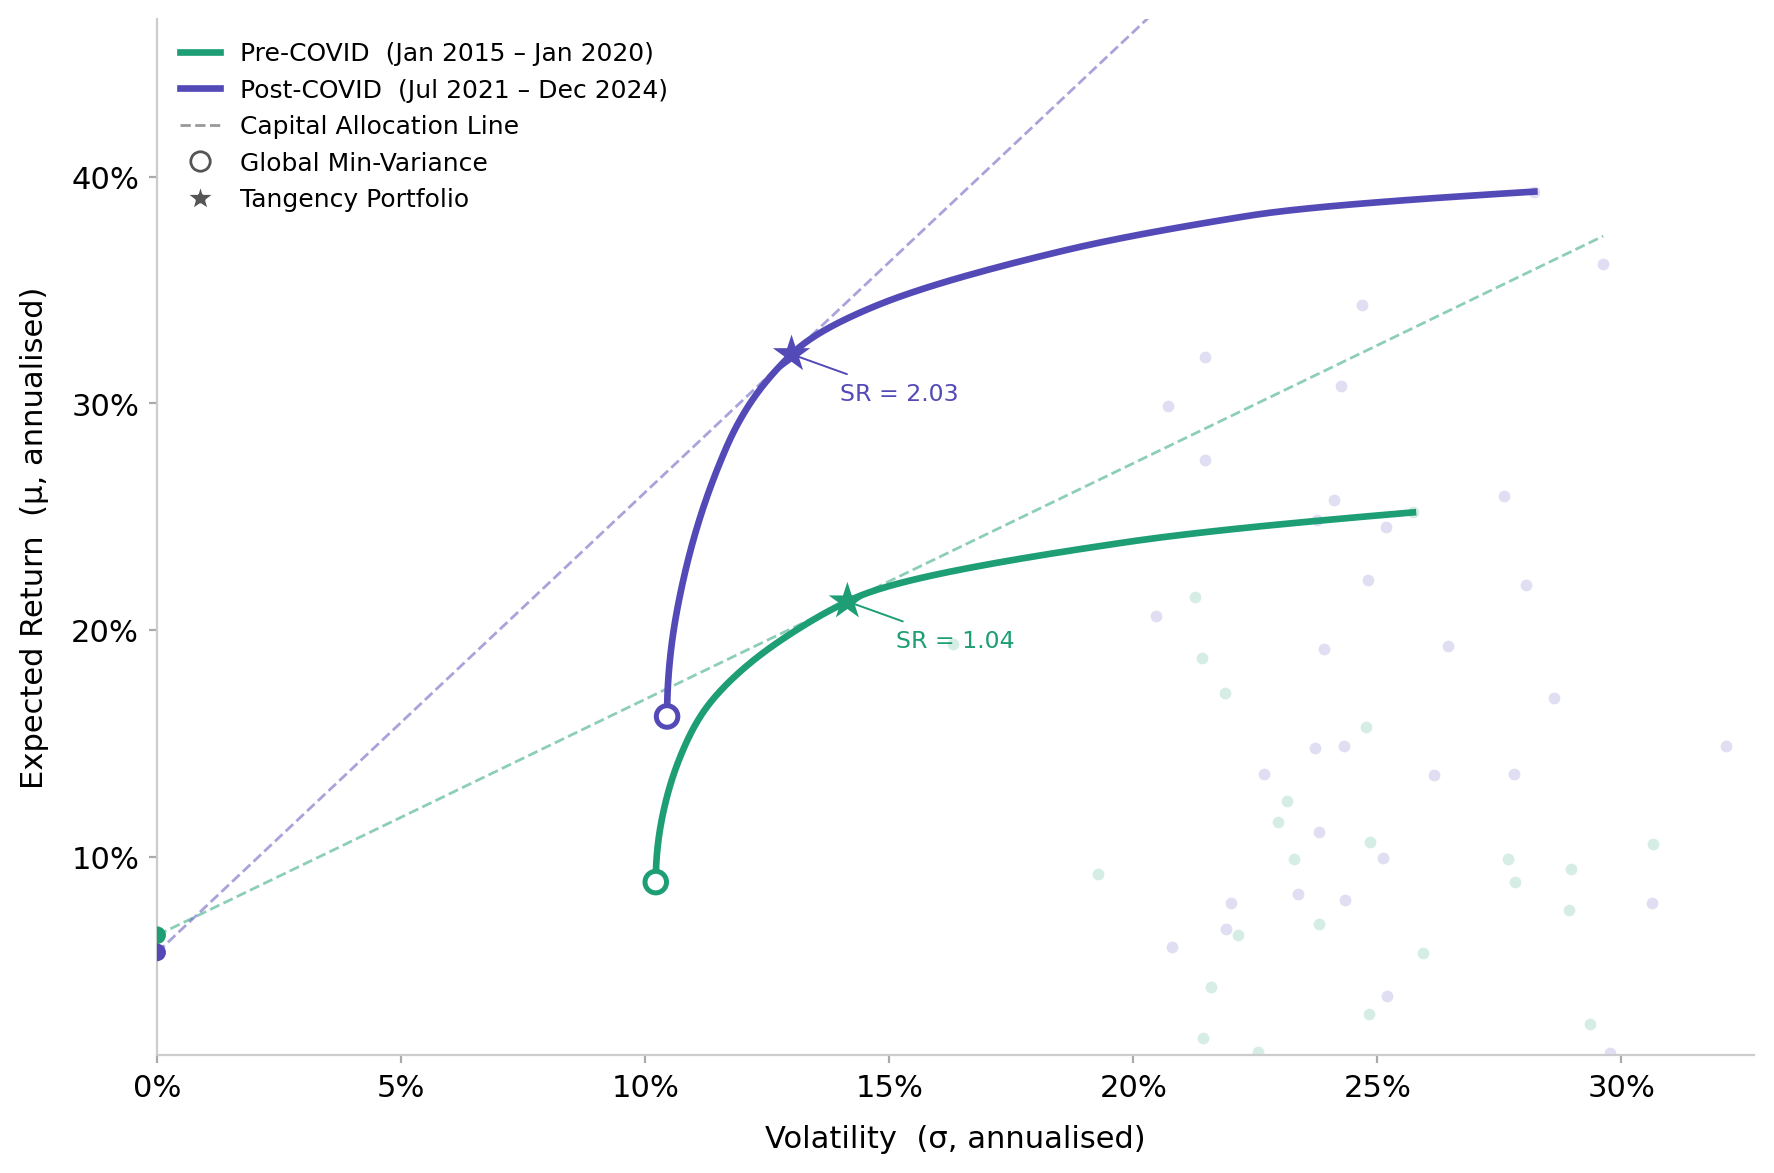
\includegraphics[width=\textwidth]{Figures/frontier_combined_weekly.png}
  \end{columns}
  \vspace{0.5em}
  \small The post-COVID frontier lies \emph{above and to the right} in both cases --- the risk-return trade-off improved materially.
\end{frame}
% ─────────────────────────────────────────────
\begin{frame}{Interpreting the Frontier Shift}
  \begin{columns}[T]
    \column{0.5\textwidth}
      \textbf{What Shifted?}
      \begin{itemize}
        \item \textbf{Northeast movement}: Higher returns \alert{and} higher volatility
        \item Return gain (+5 pp) \alert{exceeds} volatility gain (+3 pp)
        \item \textbf{Steeper CAL}: Sharpe ratio improved +6--7\% across frequencies
        \item \alert{Entire frontier} shifted, not just tangency point
      \end{itemize}

    \column{0.5\textwidth}
      \textbf{Why Returns Increased}
      \begin{itemize}
        \item Sectoral rotation into high-growth areas (pharma, tech, metals, autos)
        \item FII inflows from China+1 strategy
        \item PLI schemes boosting industrials
        \item Persistent equity risk premium expansion
      \end{itemize}
  \end{columns}

  \vspace{0.1em}
  \textbf{Why Volatility Increased (But Less Than Returns)}
  \begin{itemize}
    \item Inflation uncertainty, geopolitical shocks, Fed tightening transmitted globally
    \item \alert{But}: Correlation structure improved; sectoral dispersion was \emph{diversifiable}
    \item SIP flows dampened daily volatility in large-caps
  \end{itemize}
\end{frame}
% ─────────────────────────────────────────────
\begin{frame}{Tangency Portfolio: Sectoral Rotation}
  \begin{columns}[T]
    \column{0.55\textwidth}
      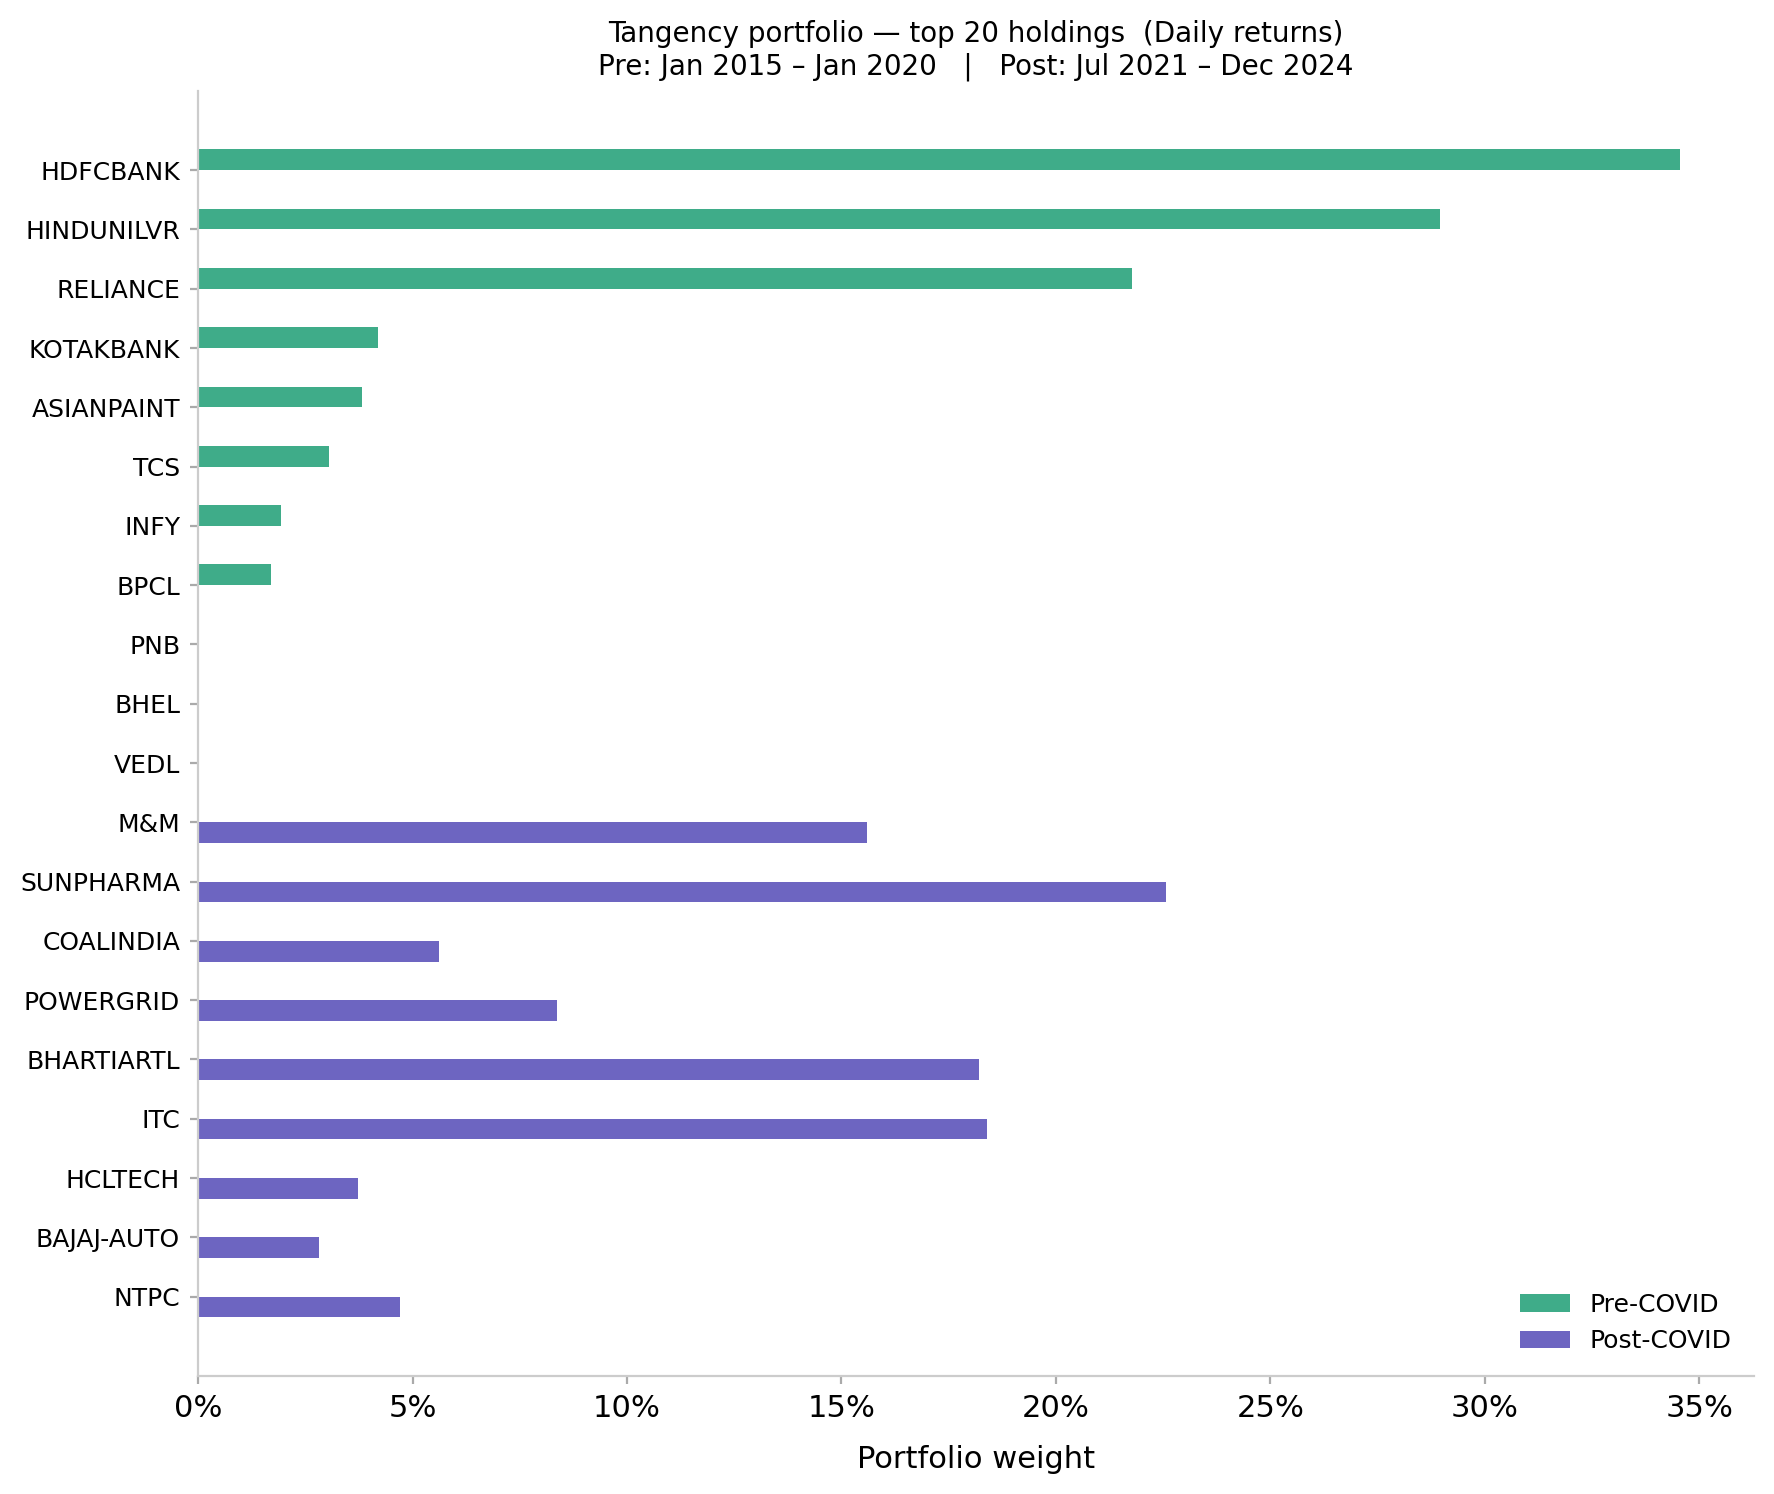
\includegraphics[width=\textwidth]{Figures/tangency_weights_daily.png}

    \column{0.42\textwidth}
      \small
      \textbf{\textcolor{precovid}{Pre-COVID top holdings}}
      \begin{itemize}\setlength\itemsep{0.1em}
        \item HDFCBANK \hfill 34.5\%
        \item HINDUNILVR \hfill 29.0\%
        \item RELIANCE \hfill 21.8\%
      \end{itemize}

      \vspace{0.2em}
      \textbf{\textcolor{postcovid}{Post-COVID top holdings}}
      \begin{itemize}\setlength\itemsep{0.1em}
        \item SUNPHARMA \hfill 22.6\%
        \item ITC \hfill 18.4\%
        \item BHARTIARTL \hfill 18.2\%
        \item M\&M \hfill 15.6\%
      \end{itemize}

      \small Complete rotation out of \textbf{financials \& FMCG} into \textbf{pharma, telecom, energy, autos}
  \end{columns}
\end{frame}

\begin{frame}{Five Structural Drivers}
  \small
  \begin{enumerate}
    \item \textbf{Monetary regime change} --- RBI accommodation expanded equity risk premia; subsequent tightening added volatility without killing returns
    \vspace{0.3em}
    
    \item \textbf{Sectoral recomposition} --- Complete rotation from financials/FMCG to pharma/tech/metals/autos; winners won \emph{bigger}
    \vspace{0.3em}
    
    \item \textbf{Correlation decline} --- Post-crisis recovery featured \alert{lower} cross-sector correlations than pre-COVID; diversification improved
    \vspace{0.3em}
    
    \item \textbf{China+1 FII flows} --- Record foreign inflows improved liquidity, compressed spreads, reduced idiosyncratic volatility
    \vspace{0.3em}
    
    \item \textbf{Retail participation surge} --- SIP flows (₹8k → ₹20k cr/month) stabilized large-cap volatility; systematic buying absorbed dips
  \end{enumerate}
  
  \vspace{0.5em}
  \centering
  \alert{These are structural, not cyclical} --- the new frontier may persist.
\end{frame}

\begin{comment}
% ─────────────────────────────────────────────
\begin{frame}{Interpreting the Shift}
  \noindent \textbf{Why did the frontier shift northeastward?}

  \begin{columns}[T]
    \column{0.5\textwidth}
      \textbf{Demand-side drivers}
      \begin{itemize}
        \item Post-COVID fiscal stimulus and infra spending (PLI schemes, BHEL, TATAPOWER)
        \item Domestic retail investor surge: Demat accounts doubled 2020--2022
        \item Foreign capital inflows as India became a China+1 alternative
      \end{itemize}

    \column{0.5\textwidth}
      \textbf{Structural / sectoral drivers}
      \begin{itemize}
        \item Cyclicals and metals outperformed on commodity supercycle (VEDL, HINDALCO, TATASTEEL)
        \item Digital transformation boosted IT returns (HCL, TCS)
        \item Pharma re-rated as strategic post-COVID (SUNPHARMA)
        \item Financials drag: regulatory tightening + HDFC-HDFCBANK merger uncertainty
      \end{itemize}
  \end{columns}
\end{frame}
\end{comment}
% ─────────────────────────────────────────────
\begin{frame}{Stock-Level: Biggest Winners}
  \centering
  \begin{tabular}{llrrl}
    \toprule
    \textbf{Ticker} & \textbf{Company} & \textbf{Pre} & \textbf{Post} & \textbf{$\Delta$} \\
    \midrule
    VEDL      & Vedanta                  & $+$8.0\%  & $+$51.2\% & \textcolor{postcovid}{+43.2 pp} \\
    TATAPOWER & Tata Power               & $-$4.9\%  & $+$48.7\% & \textcolor{postcovid}{+53.5 pp} \\
    BHEL      & Bharat Heavy Electricals & $-$20.7\% & $+$46.8\% & \textcolor{postcovid}{+67.5 pp} \\
    M\&M      & Mahindra \& Mahindra     & $+$0.4\%  & $+$43.0\% & \textcolor{postcovid}{+42.6 pp} \\
    SUNPHARMA & Sun Pharmaceutical       & $-$10.4\% & $+$34.1\% & \textcolor{postcovid}{+44.5 pp} \\
    HCLTECH   & HCL Technologies         & $+$8.6\%  & $+$32.4\% & \textcolor{postcovid}{+23.8 pp} \\
    \bottomrule
  \end{tabular}

  \vspace{0.6em}
  \small Industrials, metals, pharma, and IT led the post-COVID recovery.\\
  BHEL and TATAPOWER flipped from worst to top performers 
\end{frame}

% ─────────────────────────────────────────────
\begin{frame}{Stock-Level: Pre-COVID Stars That Faded}
  \centering
  \begin{tabular}{llrrr}
    \toprule
    \textbf{Ticker} & \textbf{Company} & \textbf{Pre} & \textbf{Post} & \textbf{$\Delta$} \\
    \midrule
    KOTAKBANK  & Kotak Mahindra Bank & $+$21.1\% & $+$4.6\%  & \textcolor{precovid}{$-$16.5 pp} \\
    HDFCBANK   & HDFC Bank           & $+$19.7\% & $+$10.6\% & \textcolor{precovid}{$-$9.1 pp}  \\
    HINDUNILVR & Hindustan Unilever  & $+$17.9\% & $+$7.9\%  & \textcolor{precovid}{$-$10.0 pp} \\
    ASIANPAINT & Asian Paints        & $+$17.8\% & $+$9.4\%  & \textcolor{precovid}{$-$8.4 pp}  \\
    BPCL       & BPCL                & $+$23.5\% & $+$15.3\% & \textcolor{precovid}{$-$8.2 pp}  \\
    \bottomrule
  \end{tabular}

  \vspace{0.6em}
  \small Financials and consumer staples --- the pre-COVID defensives --- underperformed significantly post-COVID.\\
  These are also the stocks that \emph{dominated the pre-COVID tangency portfolio}.
\end{frame}


% ─────────────────────────────────────────────
\begin{frame}{Limitations}
  \begin{itemize}
    \item \textbf{Survivorship bias} --- fixed 2015 universe excludes stocks that failed or were delisted; biases results upward
    \item \textbf{Long-only constraint} --- rules out short selling; actual attainable frontier may be wider
    \item \textbf{Transaction costs \& liquidity} --- not modeled
    \item \textbf{Causal attribution} --- the drivers discussed are correlational; isolating macro causes requires further regression analysis
  \end{itemize}
\end{frame}

% ─────────────────────────────────────────────
% \begin{frame}{Future Roadmap}
%   \begin{enumerate}
%     \item \textbf{Statistical significance test} --- bootstrap or permutation test for the frontier shift; quantify the probability that the observed gap is due to sampling noise
%     \vspace{0.4em}
%     \item \textbf{Transaction cost modeling} --- estimate rebalancing costs for the tangency portfolio; assess whether the Sharpe improvement survives after costs
%     \vspace{0.4em}
%     \item \textbf{Out-of-sample validation} --- apply post-COVID tangency weights to 2025 data; test whether the frontier shift was a durable regime change or a bull-market artifact
%   \end{enumerate}
% \end{frame}

% ─────────────────────────────────────────────
% ─────────────────────────────────────────────
\begin{frame}{Future Roadmap}
  \footnotesize
  \begin{enumerate}
    \item \textbf{Jobson-Korkie test} --- Test whether the Sharpe ratios of the pre- and post-COVID tangency portfolios are statistically different from each other, accounting for sampling uncertainty
    \vspace{0.25em}
    
    \item \textbf{De Roon \& Nijman spanning test} --- Determine if the post-COVID frontier is truly outside the pre-COVID frontier, or whether it can be spanned by the original assets with different weights
    \vspace{0.25em}
    
    \item \textbf{Frontier shift decomposition} --- Decompose the shift into mean return changes vs. covariance structure changes; isolate whether improved Sharpe ratios come from higher expected returns or better diversification
    \vspace{0.25em}
    
    \item \textbf{Covariance matrix estimation robustness} --- Compare Ledoit-Wolf shrinkage with alternative estimators (POET, factor models, DCC-GARCH); assess sensitivity of frontier position to covariance estimation method
    \vspace{0.25em}
    
    \item \textbf{Bootstrap confidence intervals} --- Construct 95\% confidence bands around both frontiers; quantify the probability that the observed gap is due to sampling noise versus a genuine structural shift
    \vspace{0.25em}
    
    \item \textbf{Transaction cost modeling} --- Estimate rebalancing costs for the tangency portfolio; assess whether the Sharpe improvement survives after accounting for bid-ask spreads and turnover
    \vspace{0.25em}
    
    \item \textbf{Out-of-sample validation} --- Apply post-COVID tangency weights to 2025 data; test whether the frontier shift was a durable regime change or a bull-market artifact
  \end{enumerate}
\end{frame}
% ─────────────────────────────────────────────
\begin{frame}[standout]
  Thank you\\[0.5em]
  \normalsize Questions?
\end{frame}

\end{document}
